\documentclass[a4paper,12pt]{article} 

\usepackage[top = 2.5cm, bottom = 2.5cm, left = 2.5cm, right = 2.5cm]{geometry} 

% packages
\usepackage{amsmath, amsfonts, amsthm} % basic math packages
\usepackage{tikz} % for making illustrations
\usetikzlibrary{shapes.arrows, arrows, decorations.markings, positioning}
\usetikzlibrary{calc}
\usetikzlibrary{3d}
\usepackage{graphicx} % for importing images
\usepackage{xcolor} % more color options
\usepackage{colortbl}
\usepackage{multicol} % for making two-column lists
\usepackage{hyperref} % for hyperlinking
%\hypersetup{colorlinks=true, urlcolor=cyan,}
\usepackage{mathabx}
\usepackage{cleveref}
\usepackage{subfig}
\usepackage{array}
\usepackage{wrapfig}
\usepackage{bbm}
\usepackage{fancyhdr}
\usepackage{algorithm, algorithmicx, algpseudocode}
\usepackage{stmaryrd}
\usepackage{physics}


% The following two packages - multirow and booktabs - are needed to create nice looking tables.
\usepackage{multirow} % Multirow is for tables with multiple rows within one cell.
\usepackage{booktabs} % For even nicer tables.

% As we usually want to include some plots (.pdf files) we need a package for that.
\usepackage{graphicx} 

% The default setting of LaTeX is to indent new paragraphs. This is useful for articles. But not really nice for homework problem sets. The following command sets the indent to 0.
\usepackage{setspace}
\setlength{\parindent}{0in}

% Package to place figures where you want them.
\usepackage{float}

% The fancyhdr package let's us create nice headers.
\usepackage{fancyhdr}

% theorems, lemmas, examples, etc.
\newtheorem{theorem}{Theorem}[section]
% \newtheorem{corollary}{Corollary}[theorem]
% \newtheorem{lemma}[theorem]{Lemma}
\newtheorem{example}[theorem]{Example}
\newtheorem{lemma}[theorem]{Lemma}
\theoremstyle{definition}
\newtheorem{definition}{Definition}[section]
\theoremstyle{remark}
\newtheorem*{remark}{Remark}
\newtheorem*{solution}{Solution}

\def\mydefb#1{\expandafter\def\csname bf#1\endcsname{\mathbf{#1}}}
\def\mydefallb#1{\ifx#1\mydefallb\else\mydefb#1\expandafter\mydefallb\fi}
\mydefallb aAbBcCdDeEfFgGhHiIjJkKlLmMnNoOpPqQrRsStTuUvVwWxXyYzZ\mydefallb

\def\mydefb#1{\expandafter\def\csname cal#1\endcsname{\mathcal{#1}}}
\def\mydefallb#1{\ifx#1\mydefallb\else\mydefb#1\expandafter\mydefallb\fi}
\mydefallb aAbBcCdDeEfFgGhHiIjJkKlLmMnNoOpPqQrRsStTuUvVwWxXyYzZ\mydefallb

%% Change this to just the normal N,Z,R,C,P,E
\def\mydefb#1{\expandafter\def\csname bb#1\endcsname{\mathbb{#1}}}
\def\mydefallb#1{\ifx#1\mydefallb\else\mydefb#1\expandafter\mydefallb\fi}
\mydefallb CEGIKNPQRST\mydefallb

\newcommand{\half}{\frac{1}{2}}
\DeclareMathOperator{\sgn}{sgn}
\DeclareMathOperator*{\argmax}{arg\,max}
\DeclareMathOperator*{\argmin}{arg\,min}
\newcommand{\matlab}{\textsc{Matlab}}


%%%%%%%%%%%%%%%%%%%%%%%%%%%%%%%%%%%%%%%%%%%%%%%%
% 3. Header (and Footer)
%%%%%%%%%%%%%%%%%%%%%%%%%%%%%%%%%%%%%%%%%%%%%%%%

% To make our document nice we want a header and number the pages in the footer.

\pagestyle{fancy} % With this command we can customize the header style.

\fancyhf{} % This makes sure we do not have other information in our header or footer.

\lhead{\footnotesize CS 581:  Homework  \# 1}% \lhead puts text in the top left corner. \footnotesize sets our font to a smaller size.

%\rhead works just like \lhead (you can also use \chead)
\rhead{\footnotesize Scott (mtscot4)} %<---- Fill in your lastnames.

% Similar commands work for the footer (\lfoot, \cfoot and \rfoot).
% We want to put our page number in the center.
\cfoot{\footnotesize \thepage} 

\begin{document}
	
	
	%%%%%%%%%%%%%%%%%%%%%%%%%%%%%%%%%%%%%%%%%%%%%%%%
	%%%%%%%%%%%%%%%%%%%%%%%%%%%%%%%%%%%%%%%%%%%%%%%%
	
	%%%%%%%%%%%%%%%%%%%%%%%%%%%%%%%%%%%%%%%%%%%%%%%%
	% Title section of the document
	%%%%%%%%%%%%%%%%%%%%%%%%%%%%%%%%%%%%%%%%%%%%%%%%
	
	% For the title section we want to reproduce the title section of the Problem Set and add your names.
	
	\thispagestyle{empty} % This command disables the header on the first page. 
	
	\begin{tabular}{p{15.5cm}} % This is a simple tabular environment to align your text nicely 
		{\large \sc CS 581:  High Performance Computing} \\
		Emory University \\ Spring 2025 \\ Prof. Tianshi Xu \\
		\hline % \hline produces horizontal lines.
		\\
	\end{tabular} % Our tabular environment ends here.
	
	\vspace*{0.3cm} % Now we want to add some vertical space in between the line and our title.
	
	\begin{center} % Everything within the center environment is centered.
		{\Large \bf Homework \# 1} % <---- Don't forget to put in the right number
		\vspace{2mm}
		
		% YOUR NAMES GO HERE
		{\bf Mitchell Scott}\\ (mtscot4) % <---- Fill in your names here!
		
	\end{center}  
	
	\vspace{0.4cm}
	
	%%%%%%%%%%%%%%%%%%%%%%%%%%%%%%%%%%%%%%%%%%%%%%%%
	%%%%%%%%%%%%%%%%%%%%%%%%%%%%%%%%%%%%%%%%%%%%%%%%
	
	% Up until this point you only have to make minor changes for every week (Number of the homework). Your write up essentially starts here.
	
	\section{Environment}
	\begin{enumerate}
		
		\item {\bf List the environment you used to run the code (Operating System, CPU, RAM, etc.) }. 
	
		\begin{solution}
			The local environment where I was running the code was on a 2022 MacBook Pro with Apple M2 chip, 8 GB of RAM running macOS Ventura 13.3. 
		\end{solution}
	\end{enumerate}
		\section{Sequential Code}
		\begin{enumerate}
			\item The performance accuracy for all code variants was \textbf{98.14\%}.
			\item The results are seen in Tab. \ref{tab:Seq}.
			\begin{table}[h]
				\centering
				\begin{tabular}{|c|l|}
					\hline
					\textbf{Trial}& \textbf{Time (ms)}  \\
					\hline\hline
					1&  3247 \\
					2&   3268\\
					3&   3288 (\textbf{high})\\
					4&    3238 (\textbf{low})\\
					5&    3273\\
					\hline
					Avg&  3262.7\\
					\hline
				\end{tabular}
				\caption{Sequential Code for model.}
				\label{tab:Seq}
			\end{table}
		\end{enumerate}
		\section{OpenMP}
		\begin{enumerate}
			\item The performance accuracy for all code variants was \textbf{98.14\%}.
			\item The results are seen in Tab. \ref{tab:OpenMP}.
			 \begin{table}[h]
				\centering
				\begin{tabular}{|c|l|l|l|l|}
					\hline
					\textbf{Trial}& \textbf{1 thread (ms)}  &\textbf{2 thread (ms)}  &\textbf{4  thread (ms)}  &\textbf{8 thread (ms)}  \\
					\hline\hline
					1& 3399 & 1768 &1015  &  710\\
					2&  3555 (\textbf{high})&1837 (\textbf{high}) &924  &  708\\
					3& 3397 & 1770 & 917 (\textbf{low}) &708  \\
					4& 3407 & 1765 (\textbf{low}) & 1035 (\textbf{high}) & 702 (\textbf{low})  \\
					5& 3391 (\textbf{low}) &1797  & 918 & 745 (\textbf{high})  \\
					\hline
					Avg& 3401 &1778.3  &952.3  & 708.7 \\
					\hline
				\end{tabular}
				\caption{OpenMP Code for model over changing thread numbers.}
				\label{tab:OpenMP}
			\end{table}
			In terms of the speedup, first we need to recall that 
			\begin{align}
				\text{Speedup} = \frac{T_{\text{sequential}}}{T_{\text{parallel}}}\label{eqn:speedup}
			\end{align}
			So simply by dividing our times from the result in section 1, the speedup is seen in Tab. \ref{tab:speedOMP}.
			\begin{table}[h]
				\centering
				\begin{tabular}{|c|c|}
					\hline
					\textbf{\# Thread}& \textbf{Speedup}  \\
					\hline\hline
					1&  0.95934 \\
					2&   1.83473\\
					4&   3.42613\\
					8&   4.60378\\\hline
				\end{tabular}
				\caption{Speedup of OpenMP for varying number of threads.}
				\label{tab:speedOMP}
			\end{table}
			\item The speedups for sequential (baseline), OpenMP, and PThreads are plotted in Fig. \ref{fig:speedup}.
			\begin{figure}[h]
				\centering
				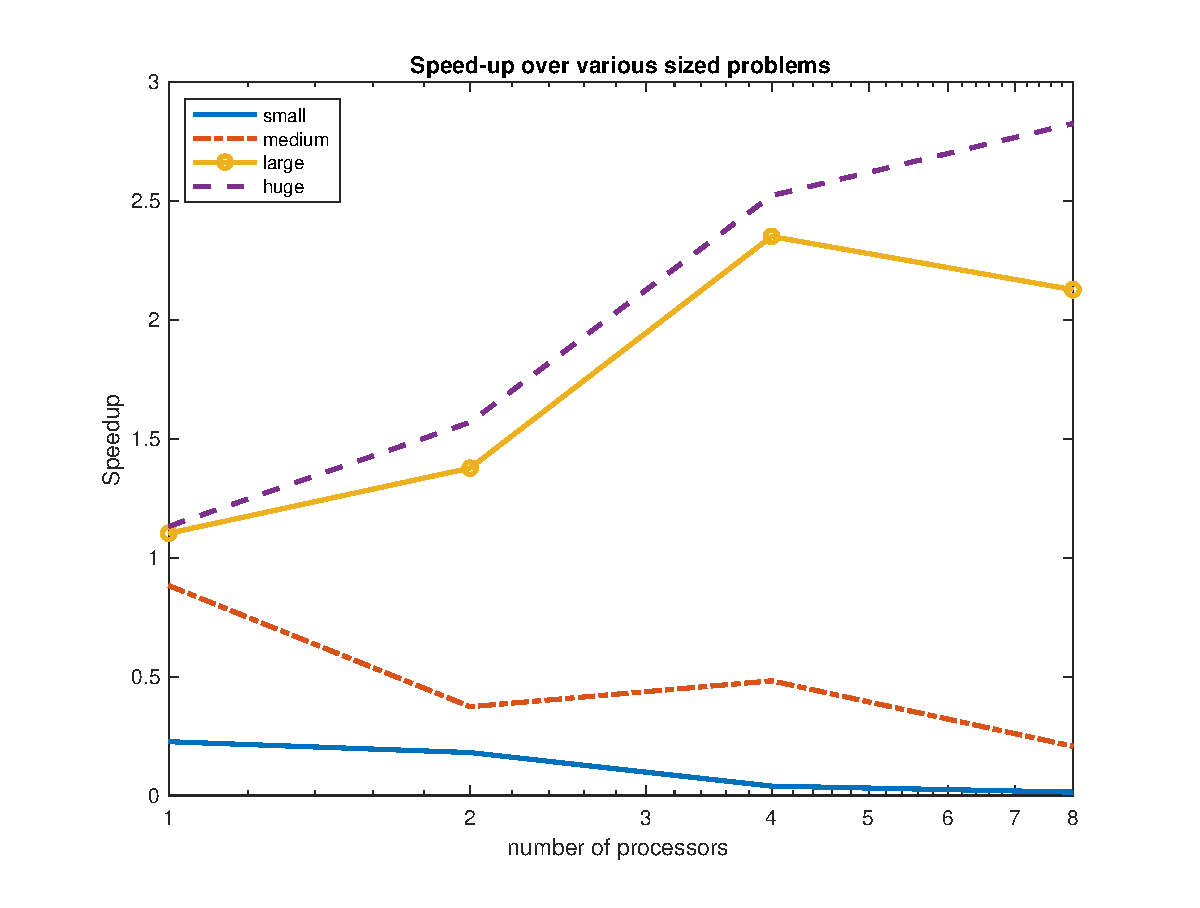
\includegraphics[width=0.7\linewidth]{speedup}
				\caption{The speedup compared to the sequential code for OpenMP and PThreads for varying threads.}
				\label{fig:speedup}
			\end{figure}
			
		\end{enumerate}
		
		\section{Pthreads}
		\begin{enumerate}
			\item The performance accuracy for all code variants was \textbf{98.15\%}.
			\item \begin{table}[h]
				\centering
				\begin{tabular}{|c|l|l|l|l|}
					\hline
					\textbf{Trial}& \textbf{1 thread (ms)}  &\textbf{2 thread (ms)}  &\textbf{4  thread (ms)}  &\textbf{8 thread (ms)}  \\
					\hline\hline
					1&  3362 (\textbf{high})& 1694 (\textbf{high}) & 866(\textbf{low}) &640  (\textbf{high})\\
					2& 3179 &1680 & 1074 (\textbf{high}) &664   \\
					3&  3128 (\textbf{low})&  1653 (\textbf{low}) &  939 & 646  \\
					4&  3175& 1685 &880  &665  \\
					5&  3138& 1664 &  870 & 683 (\textbf{high}) \\
					\hline
					Avg&  3163&1676.3  &896.3 & 658.3 \\
					\hline
				\end{tabular}
				\caption{PThread Code for model over changing thread numbers.}
				\label{tab:Ptheads}
			\end{table}
			Recalling Eq. \ref{eqn:speedup}, simply by dividing our times seen in Tab. \ref{tab:Ptheads} by the result in section 1, the speedup is seen in Tab. \ref{tab:speedPT}.
			\begin{table}[h]
			\centering
			\begin{tabular}{|c|c|}
				\hline
				\textbf{\# Thread}& \textbf{Speedup}  \\
				\hline\hline
				1&  1.03152 \\
				2&   1.94637\\
				4&   3.64019\\
				8&   4.95625\\\hline
			\end{tabular}
			\caption{Speedup of PThreads for varying number of threads.}
			\label{tab:speedPT}
			\end{table}
			\item This has already been done in Fig. \ref{fig:speedup}.
		\end{enumerate}
		\section{Implementation}
		\begin{enumerate}
			\item How do you design your sequential implementation to be cache efficient?
			\begin{solution}
				The forward pass of the algorithm is essentially solving
				\begin{align}
					\bfx_{\text{output}}&= \sigma\left(\bfW \bfx_{\text{input}} + \bfb \right), \quad \text{where}\\
					\sigma(x) &= \begin{cases}
						x,& x\geq0\\ 0, &x<0
					\end{cases}
				\end{align}
				is the ``rectified linear unit" (ReLU). The $\bfx_{\text{output}}$ is stored as a long vector of length ``output\_dim $\times$ batch\_size'', but can be thought of as a matrix stored F (as in Fortran) style. Similarly $\bfx_{\text{input}}$ has the same vector to matrix mapping but with vector of length ``input\_dim $\times$ batch\_size''. Conversely, $\bfW$ is a matrix stored as a vector of length ``input\_dim $\times$ output\_dim'', but it is stored C style, which means that performing the repeated matvec of $\bfW\bfx_{\text{input}}$ is essentially an inner product. 
				
				First we initialize $\bfx_{\text{output}}$ as a vector of floats. Then we move $\bfb$ into the cache to make repeated copies of it into the newly initialized (to zero) $\bfx_{\text{output}}$. Now that we have accounted for the bias term, we need to increment the matrix-matrix multiplication. We do this by first considering the batches, then the output, then the input. We utilize the fact that $\bfW$ is C style and $\bfx_{\text{input}}$ is F style to increment the counters to be cache efficient. 
			\end{solution}
			\item How do you parallelize the linear layer and the ReLU activation function?
			\begin{solution}
				For the OpenMP code, it was very straightforward to turn my model code into parallel code for the linear layer and ReLU function. I simply put the \#pragma omp for outside of the largest for loop. Since we are trying to parallelize nested for loops, OpenMP cleverly divies the work up behind the scenes. Since I didn't put this parallel code in the inner more for loop, we didn't have to worry about mutexes or critical regions.
				
				For the PThreads code, I once again divided up the outer-most for loop to make sure that there was no need for a mutex. Since the outer for loop was over the batches, I essentially divided the total number of batches by the number of threads to determine the start and end batches that each thread would do. On the last thread, I changed the end batches to the last batch to ensure that no batch was left undone. Since the batches are independent, the concurrent reads and writes were essentially independent processes.
				
			\end{solution}
			\item What is the performance bottleneck of your parallel implementation?
			\begin{solution}
				In an ideal world, by doubling the amount of threads that we have, the speedup would be twice as fast. However, this is not the case. This is a demonstration of the communication bottleneck. By having more threads, we still need scatter the data from the cache to new places, and while the heavy computation can be done in parallel, the data still needs to be gathered. This communication is not for free, and is why the speedup will eventually level off.
				
				Another performance bottleneck might be the load imbalance. Assume we have 15 tasks to perform on 4 processors. Each task would need to perform 3.75 tasks, but in integer division, we would have the tasks performed per processor be 3,3,3,6. This means that the last processor has to do twice the amount of work compared to the other processors. Since the entire process needs to have all processors complete, this would obviously cause a performance bottleneck.
			\end{solution}
		\end{enumerate}
		
		
	
	\section*{Acknowledgements}
	I would like to acknowledge that I worked with fellow CS 581 students Emma Hart in OH on 2-4-25. Additionally I did use the Github Copilot to expedite my code (of course I checked the work it produced before I ran it). Lastly, I use resources from the University of Michigan EECS department to figure out how to structure my PThread code.
	
\end{document}
